\documentclass[12pt]{article}
\usepackage{amsmath}
\usepackage[pdftex]{hyperref}
\usepackage{graphicx}
\begin{document}

\section {Introduction}
\begin{itemize}
\item \textbf{Training Set} : is used to tune the \textbf{parameters} of an adaptive model
	\begin{description}
		\item What about adaptive model??
		\item How to design or select an good adaptive model??
	\end{description}
\item \textbf{Learning phase} : The precise form of the function(adaptive model) is determined during the \emph{training phase}

\item \textbf{General Workflow}
	\begin{enumerate}
		\item Preprocess:
			\begin{itemize}
				\item \textbf{Normalization} : For example : transforming different size of pics to the same one.
				\item \textbf{Reduction} : Reduce dimension or quantity, to speed up comuputation. How to reduce dimension/quantity while preserving the information in those data is not easy.
			\end{itemize}
		\item Training
		\item Test : We can't train our model on all data that we have. We have to separate some of them to verify our model.
		\item Output result
	\end{enumerate}
\end{itemize}

\textbf{Classification:}
\begin{itemize}
	\item \textbf{supervised learning} : Training data comprise examples of the input vectors \underline{along with} their corresponding target vectors
		\begin{itemize}
			\item \textbf{classification}:decrete
			\item \textbf{regression}:continuous
		\end{itemize}
	\item \textbf{unsupervised learning} : Training data consists a set of input vector \textbf{x} \underline{without} any corresponding target value
		\begin{itemize}
			\item \textbf{cluster} : to discover group of similar examples
			\item \textbf{density estimation} : to determine the distribution of data within the input space.
			\item \textbf{visualization} : to project the data from a high-dimensional space down to two/three dimensions for the purpose of \emph{visualization}. Data visualization is a hot field now. Is this can be used to preprocess data set,as mention in \emph{Reduction}?
		\end{itemize}
	\item \textbf{reinforcement learning}: finding suitable actions to take in a given situation in order to maximize a reward.\\
		Make a balance of exploration and exploitation
		\begin{itemize}
			\item \textbf{exploration} : explore the unknow space.
			\item \textbf{exploitation} : make use of the actions that are known to yield a high reward.
		\end{itemize}
		Do you remember PSO ???
		\begin{equation}
		V(t+1) = w*V(t) + C_{1}*R_{1}*(P(t) - X(t)) + C_{2}*R_{2}*(G(t) - X(t))
		\end{equation}
		\begin{equation}
		X(t+1) = X(t) + V(t+1)
		\end{equation}
		It also need a balance between exploitation and exploration.But it has a global attraction when particle explore the unknown space. It is lucky...HA!
	\item \textbf{deep learning} : a new branch of machine learning. \href{http://en.wikipedia.org/wiki/Deep\_learning}{wikipedia}	
\end{itemize}

\section {Mathematica}
\paragraph{Covariance}
\begin{equation}
cov(X,Y) = E((X-\mu)(Y-\nu))
\end{equation}
Why?Why covariance is define like this?We can see what it is defined in \href{http://mathworld.wolfram.com/Covariance.html{mathworld}}:
\begin{quote}
Covariance provides a measure of the strength of the correlation between two or more sets of random variates.
\end{quote}

\begin{enumerate}
	\item It is a measure of correlation. \textbf{correlation} means two or more factors are equal. They play the role. So they should be the \textbf{same form} in covariance equation.... 
	\item It is product of the difference between item and expectation. Product is a good choice. It can refect the relationship perfectly. 
\end{enumerate}

\begin{quote}
The variance of a random variable X is its second central moment, the expected value of the squared deviation from the mean 
\end{quote}
\begin{equation}
	\sigma^2(X) = E[(X-\mu)(X-\mu)]
\end{equation}
The variance can also be thought of as the covariance of a random variable with itself:
\begin{equation}
	cov(X,Y) = E((X-\mu)(Y-\mu))
\end{equation}

\paragraph{Normal Distribution}
A normal distribution in a variate X with mean $\mu$ and variance $\sigma^2$ is a statistic distribution with probability density function
\begin{figure}[ht!]
\centering
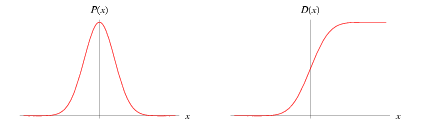
\includegraphics{./img/NormalDistribution.png}
\caption{Normal Distribution}
\end{figure}

\begin{equation}
	P(x) = \frac{1}{\sigma\sqrt{2\pi}}e^{-(x-\mu)^2/(2\sigma^2)}
\end{equation}
Why \textbf{Normal Distribution} is useful?According to \href{http://mathworld.wolfram.com/CentralLimitTheorem.html}{Central Limit Theorm}, the \textbf{mean} of any set of variates with any distribution having a finite mean and variance tends to the normal distribution. 

\begin{equation}
X_{norm}\equiv\frac{\sum_{i=1}^Nx_{i}-\sum_{i=1}^N\mu_{i}}{\sqrt{\sum_{i=1}^N}\sigma^2}
\end{equation}

Then ???Why this is useful? What $X_{norm}$ means? What is the \textbf{normal form}?


P26. What is figure 1.14 really looks like taking the consideration of $x_n=\aleph(\mu, \sigma^2)$. \\

P27. Please reason Formula 1.57 and Formula 1.58 resulting
from Formula 1.55 and Formula 1.56 respectively.
It is said $\mu_ML \sim \aleph(\mu, \sigma^2/n)$ and
$\sigma^2_{ML} \sim \frac{\sigma^2}{n}\cdot \chi^2_{n-1}$.
While $\widetilde{\sigma}^2 \sim \frac{\sigma^2}{n-1}\cdot \chi^2_{n-1}$.\\
And in the textbook, it is said that the maximum likelihood
approach systematically underestimates the variance
($\sigma^2_{ML}$) of the distribution because it is
measured relative to the sample mean and not relative
to the true mean. Can you link this statement with
the formula 1.58?\\

1.2.5 (P28-30): Both \emph{maximum likelihood function}
and \emph{maximum posterior(MAP)} methods are introduced
for the problem of polynomial curve fitting. While
in the MAP method, please reasoning the formula 1.67
from 1.66.\\

1.2.6 (P30-31): How can we get the result of formula 1.69?\\

1.3 (P32): How to make full use of the precious training data?
1) Cross-validation
2) Leave-one-out technique
3) Information criteria method

1.5.1 (P39-40): When minimizing the misclassification rate,
we should assign each value of $x$ to the class having
the higher posterior probability $p(C_k|x)$, how should
we decision the value of $x$? In Figure 1.24, it is said
the optimal value is where the curves for $p(x, C_1)$
and $p(x, C_2)$ cross. Why?

1.5.3 (P42): If there are $K$ classes then setting $\theta < 1/ K$
will ensure that no examples are rejected. That is because
$\sum^K_{i=1}p(C_k|x)=1$.

1.5.4 (P45) Compensating for class priors: Do not understand the
last half part...?


\end{document}

